\documentclass[a4paper,12pt]{scrbook} 
%%\documentclass[a4paper,12pt]{scrreprt} 
%%\documentclass[a4paper,12pt]{scrartcl} 


%Postanschrift Peter:
%
% Fujitsu Technology Solutions GmbH
% Herr Colban
% Wohlrabedamm 32
% 13629 Berlin

%%apt-get install texlive-lang-german kile kile-l10n  aspell-de%%damit ngerman keine Probleme mehr macht !!
\usepackage[utf8]{inputenc} 
\usepackage[T1]{fontenc}
\usepackage[ngerman]{babel}

%Das Paket wird für die anderthalb-zeiligen Zeilenabstand benötigt
\usepackage{setspace}


%%HTWM-Vorlage - benoetigt apt-get install texlive-fonts-extra
\setcounter{tocdepth}{2}				%Schatelungstiefe Inhaltsverz.

\usepackage[hyphens]{url} %lange URLs werden damit am Zeilenende umgebrochen
\usepackage[utf8]{inputenc}			%deutsche Umlaute
\usepackage{german, ngerman}
\usepackage[ngerman]{babel}		%Rechtschreibprüfung
\usepackage{color,listings} %Quellcode Highlighting, bindet das
\usepackage{float}					%% GRAFIKPOSITION MITTELS [H] ERWZINGEN
%Paket Listings ein
%%
\usepackage{color}
\usepackage{textcomp}
\usepackage[T1]{fontenc}				%srccode
\usepackage[scaled]{beramono}		%srccode
\usepackage{longtable}				%mehrseitige tabellen
\usepackage[tableposition=b]{caption}
\usepackage[pdftex, pdftoolbar=false, hyperfootnotes=false,bookmarks,bookmarksopen, bookmarksnumbered, bookmarksopenlevel=2,pdfpagelabels=true,pdfstartpage=1,pdfstartview=FitH]{hyperref} %PDF-Verlinkungen
\usepackage{array}					%farbige Tabellen
\usepackage[table]{xcolor} 			%farbige Tabellen
\usepackage{graphicx}				% \includegraphics bnoetigt dies

\usepackage{fancyhdr, graphicx}	

%%%%Wasserzeichen
%\usepackage{draftwatermark}			% wasserzeichen
%Quelle: http://choorucode.com/2010/05/05/latex-adding-draft-watermark/?like=1&source=post_flair&_wpnonce=1c9f85538d
%\SetWatermarkText{VORABVERSION}		% wasserzeichen-text
%\SetWatermarkLightness{0.9}			% wasserzeichen-kontrast
%\SetWatermarkScale{2.5}				% wasserzeichen-zeichengroe\ss{}e

%%%% mathemathische Formeln zentrieren und vom Text absetzenmittels \[ E = mc^2 \] anstatt $ E = mc^2 $ %%%%
\usepackage{amsmath}
\usepackage{amsthm}
\usepackage{amsbsy}
\usepackage{amssymb}


\usepackage{float} %% force image position by using big H: \begin{figure}[H]
\usepackage{datetime} %% \today zusaetzlich mit uhrzeit
%\usepackage{marginnote} %% Randnotizen, zB Bildlegende rechts auf den Rand
%\usepackage{graphicx} 	%% Bilder in Textfluss einbetten

%%%% print keyboard keys, source: http://tex.stackexchange.com/questions/5226/keyboard-font-for-latex
\usepackage{menukeys}
% use: 
%You can visualize paths \directory{/home/moose/Desktop/manual.tex} or menus \menu{View > Highlight Mode > Markup > LaTeX} or 
%key press combinations: \keys{\ctrl + \shift + F} is for formatting in Eclipse.
%You can also visualize \keys{\tab}, \keys{\capslock}, \keys{\Space}, \keys{\arrowkeyup} and many more.
%%%%%%%%%%%%%%%%%%%%%%%%%%%%%%%%%%%%%%%%%%%%%%%%%%%%%%%%%%%%%%%


\definecolor{Navy}{rgb}{0,0,0.5}
\definecolor{Gray}{gray}{0.5}
\definecolor{dunkelgrau}{rgb}{0.8,0.8,0.8}
\definecolor{hellgrau}{rgb}{0.95,0.95,0.95}
\definecolor{hellgrau2}{rgb}{0.93,0.93,0.93}
\definecolor{listinggray}{gray}{0.9}
\definecolor{lbcolor}{rgb}{0.9,0.9,0.9}

%%%%%%%%%%%%%%%%%%%%%%%%%%%%%%%%%%%%%%%%%%%%%%%%%%%%%%%%%%%%%%%%
%% print keyboard keys
%%%%%%%%%%%%%%%%%%%%%%%%%%%%%%%%%%%%%%%%%%%%%%%%%%%%%%%%%%%

\hypersetup{
	colorlinks=true, 			% false: boxed links; true: colored links
	linkcolor=Navy,          		% color of internal links
	citecolor=Gray,        			% color of links to bibliography
	filecolor=magenta,      		% color of file links
	urlcolor=blue,           			% color of external links
	linkbordercolor={1 1 1}, 		% set to white
	citebordercolor={1 1 1} 		% set to white
}


%Einrückung eines neuen Absatzes
\setlength{\parindent}{0em}

%Definition der Ränder
\usepackage[paper=a4paper,left=30mm,right=30mm,top=30mm,bottom=30mm]{geometry}

%Abstand der Fussnoten
\deffootnote{1em}{1em}{\textsuperscript{\thefootnotemark\ }}

\begin{document}

\begin{titlepage}

\begin{center}
{\huge\bfseries VoIP-Setup: FritzBox 7240 am Telekom AllIP-DSL mit Cisco 7960/7961/7962 Systemtelefonen verheiraten\par}
\vskip 1cm
\textbf{Beispielkonfiguration}
\end{center}
 
 \vfill
\vskip 3cm
\flushleft
\begin{tabular}{rl}
Von: & marcel\\ 
Am: & \today\\
\end{tabular}
\end{titlepage}

%Inhaltsverzeichnis (aktualisiert sich erst nach dem zweiten Setzen)
\tableofcontents

%Abbildungsverzeichnis und Tabellenverzeichnis auf einer Seite
%%\clearpage
\listoffigures


%%\listoftables	%% tabellnverzeichnis

%% 											\renewcommand{\lstlistlistingname}{Quellcodeverzeichnis}
\lstlistoflistings

%%  \thispagestyle{empty}
 
%Beginn einer neuen Seite
\clearpage
 
%Anderthalbzeiliger Zeilenabstand ab hier
\onehalfspacing
 
 %% ab hier Bilder mit Abb. statt Abbildung beschriften
 \renewcommand{\figurename}{Abb.}

%% Syntax Highlighting für BASH
\lstset{
	language=XML,
	keywordstyle=\bfseries\ttfamily\color[rgb]{0,0,1},
	identifierstyle=\ttfamily,
	commentstyle=\color[rgb]{0.133,0.545,0.133},
	stringstyle=\ttfamily\color[rgb]{0.627,0.126,0.941},
	showstringspaces=false,
	basicstyle=\scriptsize,
	tabsize=1,
	numbers=left,                    % where to put the line-numbers; possible values are (none, left, right)
	numbersep=5pt,                   % how far the line-numbers are from the code
	numberstyle=\tiny\color{gray}, % the style that is used for the line-numbers
	breaklines=true,	%automatischer Zeilenumbruch
	prebreak =\raisebox{0ex}[0ex][0ex]{\ensuremath{\hookleftarrow}},
	breakatwhitespace=false,
	aboveskip={1.5\baselineskip},
  	columns=fixed,
  	upquote=true,
  	extendedchars=true,
  	backgroundcolor=\color[rgb]{0.97,0.97,0.97},
}


%\pagestyle{plain}
\pagestyle{fancy}
%\renewcommand{\headrulewidth}{1pt} %Linie oben
%\fancyhf{}
%\fancyhead[L]{\nouppercase{\leftmark}} %Kopfzeile links bzw. innen
%\fancyhead[R]{\thepage} %Kopfzeile rechts bzw. außen

%\pagestyle{fancy}
%\fancyhead{}
%\fancyfoot{}
%\renewcommand{\chaptermark}[1]{\markboth{\slshape \thechapter. \ #1}{}}
%\fancyhead[LO,LE]{\leftmark}
%\fancyhead[RO,RE]{\pagemark}
%\renewcommand{\headrulewidth}{0.4pt}
%\renewcommand{\footrulewidth}{0pt}
%\fancypagestyle{plain}{%
%\fancyhf{}%
%\fancyhead[RO,RE]{\thepage}
%\renewcommand{\headrulewidth}{0pt}
%\renewcommand{\footrulewidth}{0pt}}


\pagestyle{fancy} 
\fancyhf{}  % Kopf- und Fußzeile leeren 
\renewcommand{\headrulewidth}{1pt} 
\fancyhead[EL]{\nouppercase{\leftmark}} %Kopfzeile linker Bereich auf geraden Seiten
\fancyhead[OR]{\nouppercase{\leftmark}} %Kopfzeile rechter Bereich auf ungeraden Seiten
\fancyfoot[EL]{\thepage} %% Seitenzahl links auf geraden Seiten
\fancyfoot[OR]{\thepage} %% Seitenzahl rechts auf ungeraden Seiten



\clearpage
\chapter{Einleitung}
\label{sec:0}
Dieses Dokument beschreibt mein privates Telefoniesetup zu Hause. Da es mich ein wenig Zeit gekostet hat die einzelnen Komponenten
so zum Zusammenspiel zu bewegen, möchte ich den Weg hiermit dokumentieren

\chapter{Hardware}
\label{sec:1}

Die eingesetzte Hardware untergliedert sich in drei Kathegorien und setzt sich wie folgt zusammen:

\begin{itemize}
 \item Router (stellt DSL-Verbindung her und dient als DHCP-Server für das LAN):
 \begin{itemize}
  \item IGEL UD3-H700C mit Intel Dual Gigabit Netzwerkkarte, daran Allnet ALL0333C DSL-Modem, Software: pfSense
 \end{itemize}
 \item VoIP-Server: 
 \begin{itemize}
  \item ausgediente FritzBox 7240 (DSL-Modem und WLAN defekt, Telefonieteil augenscheinlich noch funktionstüchtig)
 \end{itemize}
 \item VoIP:-Endgeräte:
 \begin{itemize}
  \item 1x LG Nexus 5 nativer Android VoIP Client
  \item 1x Siemens S685IP VoIP-DECT Basisstation
  \item 1x Cisco 7960 Systemtelefon mit SIP-Firmware
  \item 4x Cisco 7961 Systemtelefon mit SIP-Firmware
  \item 2x Cisco 7962 Systemtelefon mit SIP-Firmware
 \end{itemize}
\end{itemize}

\section{Router}
Als Router setze ich einen Thinclient von Igel ein. Das verwendete Modell UH3-H700C hat keine bewglichen Teile, 
man kann sowohl CF-Karten als auch 2,5``-IDE-Platten verbauen und das wichtigste: es gibt einen vollwertigen PCI-Steckplatz.
In diesem sitzt eine Intel Dual-Gigabit Netzwerkkarte. Beide Komponenten habe ich sehr günstig (jeweils unter 20 Euro) beim
Auktionshaus meines Vertrauens erstanden. Der Igel kommt mit einem 12V Netzteil und sollte nicht signifikant mehr Energie
verbrauchen als andere Router

Als Software setze ich pfSense ein, eine Router-Distribution auf Basis von FreeBSD. pfSense selbst bietet extrem viele Möglichkeiten,
für mich interessant ist der sehr flexibel konfigurierbare DHCP-Server und vor allem lässt sich aus der Weboberfläche sehr leicht
ersehen welche lokale IP-Adresse gerade wieviel Internet-Bandbreite belegt - für schwachbrüstige DSL-Anschlüsse wie meinen ein, ein 
wesentliches Diagnosemittel. 

Der Igel macht bei mir wirklich nur die DSL-Einwahl, WLAN und VoIP beispielsweise machen bei mir separate Geräte, dazu später mehr.
Die Lösung Igel+pfSense setze ich jetzt seit Jahren ein und mein Fazit ist bisher: rockstable.

Weiterer wichtiger Punkt: die komplette Konfiguration lässt sich als XML-Datei exportieren.

\section{VoIP-Server}
Als VoIP-Server kann man prinzipiell neben Fertigprodukten wie beispielsweise von AVM oder Lancom auch selbst VoIP-Installationen aufsetzen.
Es gibt hierzu diverse Distributionen auf Basis von Asterisk wie beispielsweise die Distributionen AsteriskNow oder FreePBX. Aber das schien mir
für meine privaten Zwecke dann doch Overkill. Außerdem möchte ich da keinen großen Wartungsaufwand bei der Telefonanlage.

\subsection{Fritzbox 7240 als VoIP-Server}
Bei einem Bekannten konnte ich eine AVM FritzBox 7240 vor der Verschrottung retten, an der nach einem Gewitter das DSL-Modem sowie 
WLAN ausgefallen waren. Die FritzBox wird so konfiguriert das sie eine lokale IP-Adresse aus dem LAN erhält und das Internet über den
IGEL-Router mit benutzt. Am Igel sind die relevanten Ports für VoIP an die FritzBox weitergeleitet. Dazu später mehr.

Wie beim IGEL-Router auch, lässt sich auch bei der FritzBox die komplette Konfiguration als XML-Datei sichern.


\section{VoIP-Clients}
Das ganze Projekt ist aus dem Wunsch heraus entstanden, neben den Mobilteilen, die durch die Siemens S685IP versorgt werden auch wieder ein
''Festnetztelefon`` zur Verfügung zu haben. Über das Auktionshaus meiner Wahl bin ich dann auf das Cisco 7960 aufmerksam geworden. Zunächst
skeptisch ob der SCCP-Firmware, habe ich das Ding erstanden. Da es nach etwas Gefummel sowohl von der Haptik als auch von der Sprachqualität 
überzeugt hat, habe ich noch ein paar Nachfolgemodelle 7961 und 7962 erstanden. Wenn man den Konfigurations- und Updatevorgang einmal prinzipiell
verstanden hat, ist es trivial eine fast beliebige Anzahl weiterer solcher Modelle in Betrtieb zu nehmen. 

\chapter{Konfiguration}
In unserem Szenario haben wir folgende Geräte:
\begin{itemize}
 \item[IP 192.168.1.1]  IGEL-Router stell Internetverbindung her und dient als DHCP-Server
 \item[IP 192.168.1.80] FritzBox als interner VoIP-Server
 \item[IP 192.168.1.91] Nexus 5 als VoIP Client mit interner Rufnummer 620 und Passwort 1234
 \item[IP 192.168.1.81] Siemens S685IP als VoIP Client mit interner Rufnummer 621 und Passwort 1234
 \item[IP 192.168.1.82] Cisco 7960 als VoIP Client mit interner Rufnummer 622 und Passwort 1234
 \item[IP 192.168.1.83] Cisco 7961 als VoIP Client mit interner Rufnummer 623 und Passwort 1234
\end{itemize}

\section{Router}
Am Router selbst ist nichts zu beachten, solange eine zuverlässige Internetverbindung besteht und die passenden Ports zum VoIP-Server durchgereicht werden.
Das sind in meinem Fall folgende Ports:
\begin{itemize}
 \item Ports 3478 bis 3480 TCP+UDP
 \item Ports 5060 bis 5080 UDP
 \item Ports 30000 bis 31000 UDP
 \item POrts 40000 bis 41000 UDP
\end{itemize}

Diese muss man per NAT zur lokalen IP-Adresse des VoIP-Servers durchreichen.

Falls man pfSense einsetzt, sollte man beim erstellen der Portregeln darauf achten, dass man 
unten bei ''filter rule association`` die Standardvorgabe in ''pass`` umändert. Weiterhin sollte man sich
dieses Dokument \footnote{\url{https://doc.pfsense.org/index.php/VoIP_Configuration}} verinnerlichen, da
beispielsweise mit der standardmäßig aktivierten Option ''source port randomization`` kein stabiler VoIP-Betrieb 
zu machen ist.

\section{VoIP-Server}
Am VoIP-Server, also der FritzBox gibt es nun zwei Bereiche die man abarbeiten muss. Ein Teil ist die Registrierung der externen SIP-Nummern,
die man von seinem Anbieter zur Verfügung gestellt bekommen hat. In meinem Fall handelt es sich um 3 SIP-Nummern an einem AllIP-Anschluss der Telekom.
Der zweite Bereich ist die Konfiguration der FritzBox als SIP-Server für die internen SIP-Telefone.

Netter Nebeneffekt wenn man die FritzBox als VoIP-Server verwendet: falls man ein GMail-Konto hat, kann man seine Kontakte vom GMail-Konto direkt in die FritzBox importieren.
\subsection{Externe SIP-Accounts}
Hier hat man mit der FritzBox und dem mitgelieferten Assistenten wirklich leichtes Spiel. Man klickt sich durch den Telefonieassistenten, indem man seinen 
VoIP-Anbieter auswählt und noch die passenden Zugangsdaten einträgt. Danach sollte die FritzBox die SIP-Nummern porblemlos registrieren können. 

\subsection{Interne SIP-Accounts}
Nun müssen wir noch für jedes interne Telefon einen SIP-Account anlegen. Das ist ebenso einfach wie im vorherigen Schritt. Man fügt in der Weboberfläche 
der FritzBox neue Telefoniegeräte hinzu. Diese bekommen die Nummern 610 und aufstreigend zugewiesen. Als Passwort empfiehlt sich für die Testphase etwas 
unkompliziertes wie 1234 zu wählen, da einige ältere Telefone sich unter Umständen nicht an der FritzBox anmelden können, falls das Passwort zu komplex ist.
Solche Probleme sind dann nur sehr schwer zu diagnostizieren. Im letzten Schritt, wenn alles so läuft wie gewünscht, sollte man natürlich sämtliche Passwörter
durch sichere Passwörter ersetzen.


\section{VoIP-Clients}
In diesem Kapitel beschreibe ich die Konfiguration meiner VoIP-Endgeräte im Haushalt, die sich dann an der FritzBox per SIP anmelden. Ich empfehle im LAN nur mit statischen
IP-Adressen zu arbeiten und sich nicht blind auf das lokale DNS zu verlassen. Zusätzlich hinterlege ich im IGEL-Router noch für die jeweilige MAC-Adresse eines Geräte die 
IP im DHCP-Server. So kann man die Geräte auch per DHCP konfigurieren lassen und es kommt trotzdem nicht zu IP-Problemen.

\subsection{LG Nexus 5}
Google's Betriebssystem Android bringt seit Version 4.2 einen nativen SIP-Client mit. Dieser eignet sich gut für erste Tests. Das zugehörige Optionsmenü ist jedoch sehr versteckt.
Man geht über die Telefon-App $\rightarrow$ Einstellungen $\rightarrow$ Anrufe $\rightarrow$ Anrufkonten $\rightarrow$ SIP-Konten. Um per SIP auch Anrufe empfangen zu können muss
das WLAN häufig genutzt werden, was sehr zu Lasten des Akkus geht.

Nun fügt man einen neuen SIP-Account hinzu:
\begin{itemize}
 \item Nutzername: <interne Rufnummer die man in der FritzBox für diesen Account gewählt hat> zB 620
 \item Passwort: <zugehöriges Passwort> zB 1234
 \item: Server: <lokale IP der FritzBox> zB 192.168.1.80
\end{itemize}

\begin{figure}[H]
\begin{center}
%\includegraphics[width=.5\hsize]{./images/informationweek-virtualizationbycathegory.png}
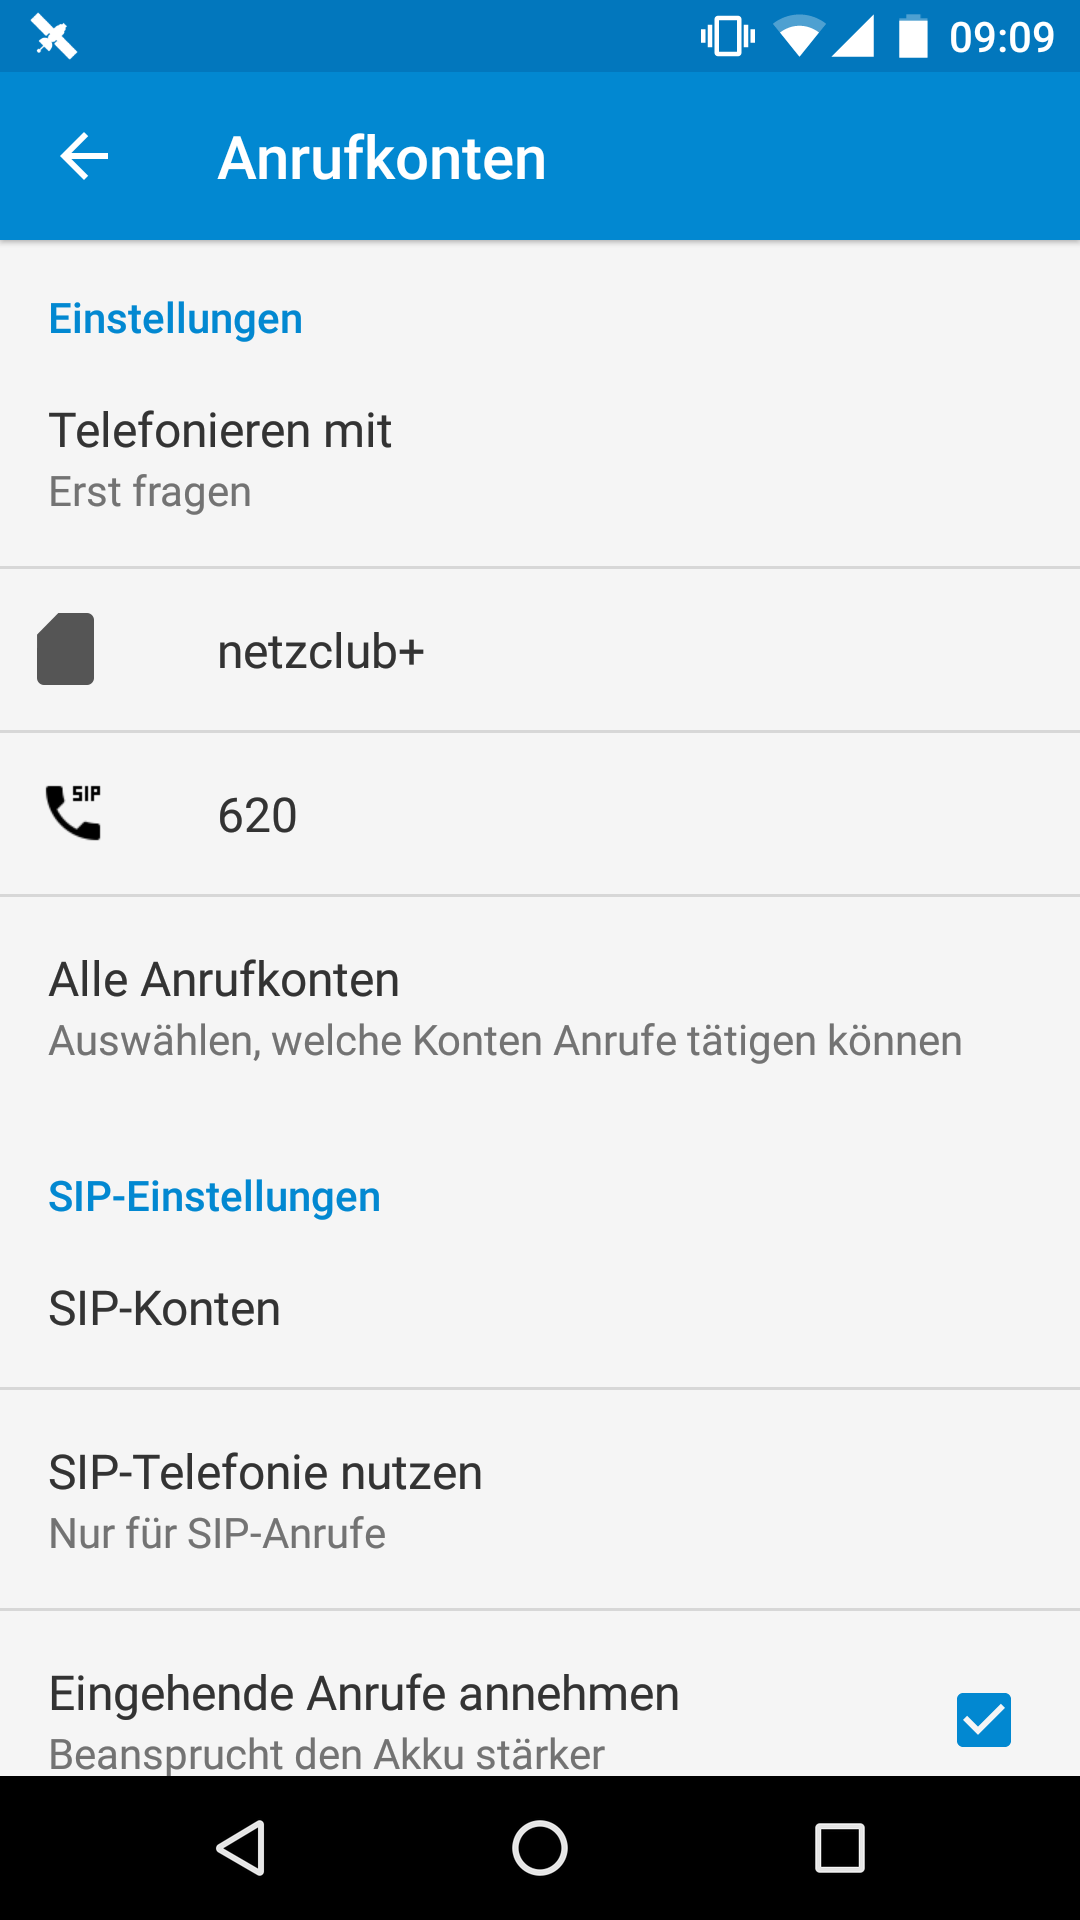
\includegraphics[width=.4\hsize]{./images/voip-client-nexus5.png}
\end{center}
\caption[Konfiguration eines SIP-Accounts in Android 5]
{\label{voip-client-nexus5}Konfiguration eines SIP-Accounts in Android 5. Quelle:Autor}
\end{figure}


Nun sollte sich das Telefon an der FritzBox anmelden können und ein- und ausgehende Gespräche möglich sein.

\subsection{Siemens S685IP}
Die Konfiguration der DECT-Basis erfolgt analog zum Nexus 5. indem man 

\begin{figure}[H]
\begin{center}
%\includegraphics[width=.5\hsize]{./images/informationweek-virtualizationbycathegory.png}
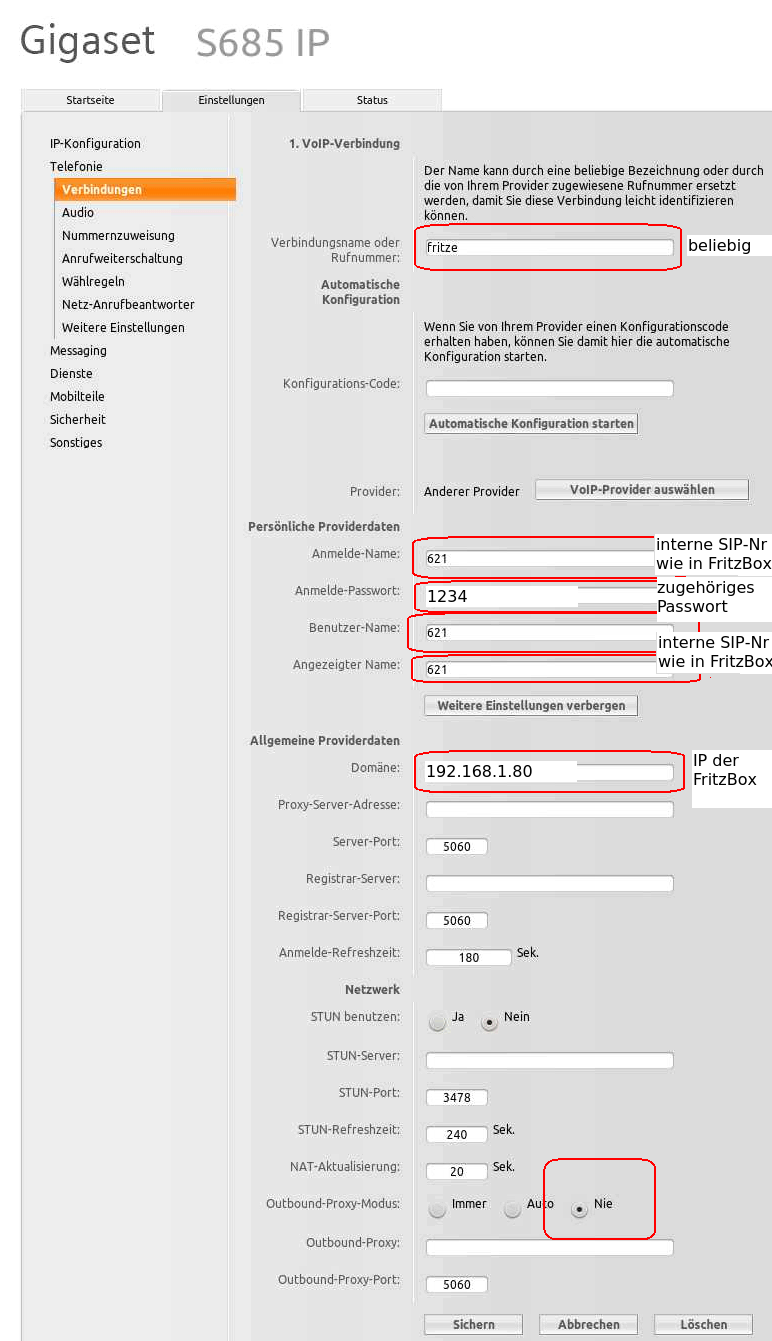
\includegraphics[width=.8\hsize]{./images/voip-client-s685ip-01.png}
\end{center}
\caption[Konfiguration eines SIP-Accounts in der DECT-Basis Siemens S685IP]
{\label{voip-client-nexus5}Konfiguration eines SIP-Accounts in der DECT-Basis Siemens S685IP. Quelle:Autor}
\end{figure}

Wenn man den Account wie im Bild angelegt hat, erscheint oft direkt eine Fehlermeldung ''Anmeldung nicht möglich`` oder ähnlich klingend.
Davon sollte man sich nicht verunsichern lassen, die DECT-Basis regiert generell ser träge im Bezug auf die Weboberfläche und braucht daher
auch zur Anmeldung an der FritzBox einige Sekunden, also Geduld. Weiterhin sollte man noch die EInstellungen wie im folgenden Bild anpassen, falls
die Registrierung an der FritzBox dauerhaft fehlschlägt.

\begin{figure}[H]
\begin{center}
%\includegraphics[width=.5\hsize]{./images/informationweek-virtualizationbycathegory.png}
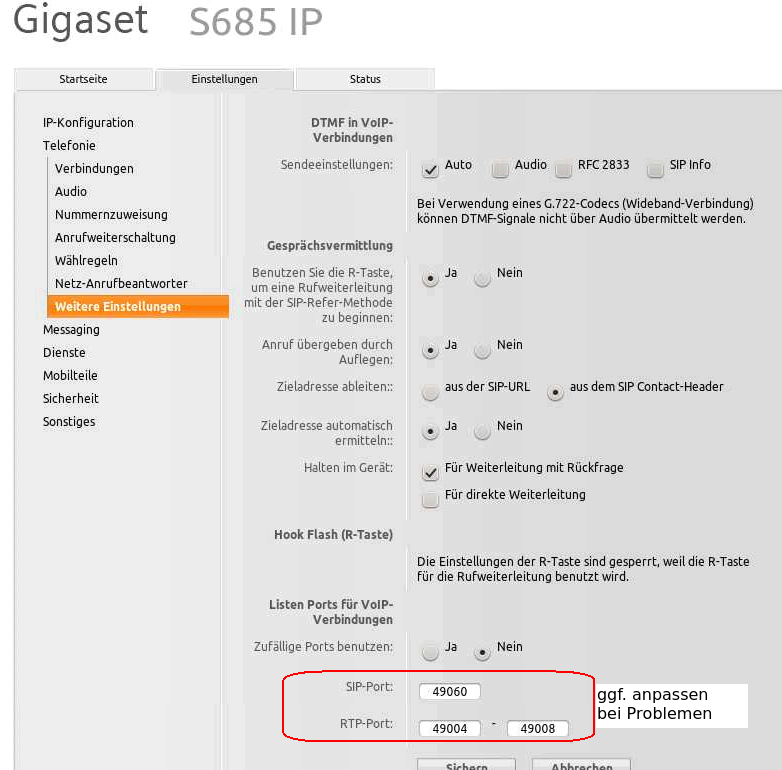
\includegraphics[width=.8\hsize]{./images/voip-client-s685ip-02.png}
\end{center}
\caption[Konfiguration eines SIP-Accounts in der DECT-Basis Siemens S685IP - weitere Einstellungen.]
{\label{voip-client-nexus5}Konfiguration eines SIP-Accounts in der DECT-Basis Siemens S685IP - weitere Einstellungen. Quelle:Autor}
\end{figure}

Anmerkung zum S685IP ansich: auch wenn die Weboberfläche einiges an Geduld erfordert, so hat sich das S685IP in 5 Jahren Benutzung als sehr zuverlässig 
erwiesen und die Investition von damals 130 Euro kann als gerechtfertigt angesehen werden. Auch die Reichweite ist im Vergleich zum DECT-Teil einer FritzBox
7270 mindestens doppelt so hoch. Wenn man nicht soviel Geld ausgeben möchte, kann man sich beim Auktionshaus seiner Wahl auch ein T-Home Sinus-501-V holen, dass
ist im Prinzip eine umgelabelte S6885IP. Einziger Unterschied zur ''echten`` S685IP ist das die Weboberfläche in magenta gehalten ist und der Festnetzanschluss (analog)
weggelassen wurde.

\subsection{Cisco 7960}
Das Cisco 7960 ist ein älteres, aber qualitativ hochweriges Systemtelefon mit, welches standardmäßig mit Ciscos proprietärem SCCP-Protokoll daher kommt. Da meines Wissens nur die Cisco Call Manager dieses Protokoll 
sprechen, muss dem Telefon erstmal eine SIP-Firmware untergeschoben werden. Das 7960 in unserem Beispiel soll die MAC-Adresse 00:12:34:56:78:ab haben, damit das Prinzip klar wird. Die echte Adresse steht hinten auf dem Telefon auf 
einem Aufkleber. 

Wir haben nun also 2 Schritte vor uns. Erstens müssen wir die Konfigurationsdateien anlegen, damit diese für unser Setup passen. Zweitens müssen wir die SIP-Firmwaredateien sowie die erstellten Konfigurationsdateien 
auf das Telefon befördern, damit dieses mit der FritzBox arbeiten kann.

\subsubsection{Konfigurationsdateien für das Cisco 7960 erstellen}

Die aktuellste SIP-Firmware für das 7960 liefert Cisco in einem Zip-File namens P0S3-8-12-00.zip welches man über eine kostenlose Registrierung
direkt bei Cisco oder durch geschicktes googlen finden kann. Wenn man die Zip-Datei entpackt erhält man folgende Dateien:
\begin{itemize}
 \item OS79XX.TXT
 \item P003-8-12-00.bin
 \item P003-8-12-00.sbn
 \item P003-8-12-00.loads
 \item P003-8-12-00.sb2
\end{itemize}

Neben diesen Dateien müssen wir jetzt noch weitere Dateien in diesem Verzeichnis anlegen:

\begin{lstlisting}[caption={SIPDefault.cnf},label=lst:7960sipdefaultcnf]
image_version: P0S3-8-12-00
proxy1_address: "192.168.1.80"   ; Can be dotted IP or FQDN
proxy2_address: ""              ; Can be dotted IP or FQDN
proxy3_address: ""              ; Can be dotted IP or FQDN
proxy4_address: ""              ; Can be dotted IP or FQDN
proxy5_address: ""              ; Can be dotted IP or FQDN
proxy6_address: ""              ; Can be dotted IP or FQDN
proxy_register: 1
messages_uri:   "1"
phone_password: "1234" ; Limited to 31 characters (Default - cisco)
sntp_mode: unicast
sntp_server: "192.168.1.1" 
time_zone: "CET" ; assuming you are in central europe
time_format_24hr: 1 ; to show the time in 24hour format
date_format: "D/M/Y"  ; format you would like the date in
\end{lstlisting}

\begin{lstlisting}[caption={XMLDefault.cnf.xml},label=lst:7960sipdefaultcnf]
<Default>
  <callManagerGroup>
     <members>
        <member priority="0">
           <callManager>
              <ports>
                 <ethernetPhonePort>2000</ethernetPhonePort>
                 <mgcpPorts>
                    <listen>2427</listen>
                    <keepAlive>2428</keepAlive>
                 </mgcpPorts>
              </ports>
              <processNodeName></processNodeName>
           </callManager>
        </member>
     </members>
  </callManagerGroup>
  <loadInformation7  model="Cisco 7960">P0S3-8-12-00</loadInformation7>
 <authenticationURL></authenticationURL>
 <directoryURL></directoryURL>
 <idleURL></idleURL>
 <informationURL></informationURL>
 <messagesURL></messagesURL>
 <servicesURL></servicesURL>
</Default>
\end{lstlisting}

In den folgenden beiden Konfigurationsdateien besteht ein Teil des Dateinamens aus der MAC-Adresse des Telefons, in unserem Beispiel lautet die MAC-Adresse des Telefons 00:12:34:56:78:ab.
Die beiden noch fehlenden Dateien für dieses Telefon heißen somit:
\begin{itemize}
 \item SEP\textbf{0012345678AB}.cnf.xml
 \item SIP\textbf{0012345678AB}.cnf
\end{itemize}
und haben folgenden Inhalt:

\begin{lstlisting}[caption={SEP0012345678AB.cnf.xml},label=lst:7960sep0012345678abcnfxml]
<device>
<loadInformation model="IP Phone 7960">P0S3-8-12-00</loadInformation>
</device>
\end{lstlisting}

\begin{lstlisting}[caption={SIP0012345678AB.cnf},label=lst:7960sip0012345678abcnf]
image_version: P0S3-8-12-00
line1_name: 622
line1_authname: "622"
line1_shortname: "622" ; displayed on the phones softkey
line1_password: "1234"
line1_displayname: "622"; the caller id
proxy1_port: 5060
proxy1_address: 192.168.1.80
# Phone Label (Text desired to be displayed in upper right corner)
phone_label: "Werkstatt " ; add a space at the end, looks neater
phone_password: "1234" ; Limited to 31 characters (Default - cisco)
user_info: none
telnet_level: 2
logo_url: "http://192.168.1.203/cisco/asterisk-tux.bmp"
\end{lstlisting}

Nun sollten sich in dem Verzeichnis die folgenden Dateien befinden:
\begin{itemize}
 \item OS79XX.TXT  
 \item P003-8-12-00.bin  
 \item P003-8-12-00.sbn  
 \item P0S3-8-12-00.loads
 \item P0S3-8-12-00.sb2
 \item SEP0012345678AB.cnf.xml
 \item SIP0012345678AB.cnf
 \item SIPDefault.cnf
\end{itemize}
Wenn alles klappt sollte sich das Telefon nach dem Update in einer Minimalkonfiguration befinden, also sich an der FritzBox anmelden und ein- und ausgehende Gespräche möglich sein.

\subsubsection{Konfigurationsdateien per TFTP auf das Cisco 7960 übertragen}
Um die Dateien aus dem vorherigen Kaptiel auf das Telefon zu bekommen, muss man einen TFTP-Server installieren. 
Ich habe hier einen Ubuntu-Server verwendet auf dem ich den atftp installiert habe:

\lstset{
	language=BASH,
	keywordstyle=\bfseries\ttfamily\color[rgb]{0,0,1},
	identifierstyle=\ttfamily,
	commentstyle=\color[rgb]{0.133,0.545,0.133},
	stringstyle=\ttfamily\color[rgb]{0.627,0.126,0.941},
	showstringspaces=false,
	basicstyle=\scriptsize,
	tabsize=1,
	numbers=left,                    % where to put the line-numbers; possible values are (none, left, right)
	numbersep=5pt,                   % how far the line-numbers are from the code
	numberstyle=\tiny\color{gray}, % the style that is used for the line-numbers
	breaklines=true,	%automatischer Zeilenumbruch
	prebreak =\raisebox{0ex}[0ex][0ex]{\ensuremath{\hookleftarrow}},
	breakatwhitespace=false,
	aboveskip={1.5\baselineskip},
  	columns=fixed,
  	upquote=true,
  	extendedchars=true,
  	backgroundcolor=\color[rgb]{0.97,0.97,0.97},
}
\begin{lstlisting}[caption={Installation von atftp unter ubuntu},label=lst:atftpdinstall]
$ sudo apt-get update

$ sudo apt-get install atftpd
$ sudo apt-get remove xinetd

$ sudo mkdir /srv/tftp && sudo chown nobody.nogroup /srv/tftp
$ sudo touch /var/log/atftpd.log  && sudo chown nobody.nogroup /var/log/atftpd.log
\end{lstlisting}

Anschließend sind noch Modifikationen an der Konfigurationsdatei /etc/default/atftpdvon atftpd nötig, damit dieser selbstständig (ohne xinetd) und mit aktiviertem Logging
lauffähig ist. In der Logdatei kann man dann während des Updatevorgangs gut sehen ob und welche Telefone sich Dateien vom atftpd abholen.

\begin{lstlisting}[caption={atftpd-Konfigurationsdatei /etc/default/atftpd},label=lst:atftpdconfig]
USE_INETD=false
OPTIONS="--tftpd-timeout 300 --retry-timeout 5 --mcast-port 1758 --mcast-addr 239.239.239.0-255 --mcast-ttl 1 --maxthread 100 --verbose=6 --logfile /var/log/atftpd.log /srv/tftp"
\end{lstlisting}

Im letzten Schritt kopieren wir noch die im vorherigen Kapitel angelegten Dateien für das 7960 in das Stammverzeichnis des atftpd, nämlich /srv/tftp und passen die Berechtigungen an:
\begin{lstlisting}
$ cd /Verzeichnis/in/dem/die/Cisco7960/Dateien/liegen
$ sudo cp * /srv/tftp/
$ sudo chmod 660 /srv/tftp/*
$ sudo chown -R nobody.nogroup /srv/tftp
\end{lstlisting}

Am Ende sollte dieses Verzeichnis so aussehen:

\begin{lstlisting}
m@marlap01:~$ ls -hal /srv/tftp/
insgesamt 1,0M
drwxr-xr-x 2 nobody nogroup 4,0K Jan 14 10:47 .
drwxr-xr-x 3 root   root    4,0K Jan 14 10:47 ..
-rw-rw---- 1 nobody nogroup   15 Jan 14 10:47 OS79XX.TXT
-rw-rw---- 1 nobody nogroup 128K Jan 14 10:47 P003-8-12-00.bin
-rw-rw---- 1 nobody nogroup 128K Jan 14 10:47 P003-8-12-00.sbn
-rw-rw---- 1 nobody nogroup  458 Jan 14 10:47 P0S3-8-12-00.loads
-rw-rw---- 1 nobody nogroup 739K Jan 14 10:47 P0S3-8-12-00.sb2
-rw-rw---- 1 nobody nogroup   89 Jan 14 10:47 SEP0012345678AB.cnf.xml
-rw-rw---- 1 nobody nogroup  535 Jan 14 10:47 SIP0012345678AB.cnf
-rw-rw---- 1 nobody nogroup  718 Jan 14 10:47 SIPDefault.cnf
m@marlap01:~$ 
\end{lstlisting}
Wenn man nun abschließend mittels

\begin{lstlisting}
$ sudo service atftpd restart
\end{lstlisting}

den atftpd noch dazu bringt die neue Konfiguration zu übernehmen, sollte der TFTP Server bereit sein. Nun ist noch dafür zu sorgen,
dass das Telefon weiß, unter welcher lokalen IP-Adresse es den TFTP-Server erreichen kann. Ich habe dazu einfach in meinem DHCP-Server
auf dem IGEL-Router als DHCP-Option die IP-Adresse des TFTP-Servers angegeben. Man kann wohl auch manuell im Telefon unter Netzwerkeinstellungen
eine IP-Adresse für den TFTP-Server angeben, dass hab ich jedoch selbst nicht ausprobiert.

\subsubsection{Cisco 7960 updaten}
Da nun alles vorbereitet ist holen wir zum Radikalschlag aus: Wir müssen die Firmware des Telefons komplett platt machen. In Folge dessen wersucht das
Telefon dann per TFTP eine neue Firmware und Konfiguration vom angegebenen TFTP-Server zu laden und bekommt diesmal die SIP-Firmware untergeschoben.

Um den Firmware-Reset durchzuführen müssen wir das 7960 vom Strom trennen. Dann wird der Strom wieder verbunden und direkt danach die Rautetaste \# gedrückt gehalten.
Wir halten \# solange gedrückt, bis die drei Tasten rechts unten abwechselnd anfangen zu blinken. Indem wir jetzt die Tasten 1 2 3 4 5 6 7 8 9 * 0 \# drücken starten wir den
Firmwarereset mit anschließendem Update. Zur Fehlerdiagnose sollte man die LOG-Datei des TFTP-Servers beobachten. Ich hatte anfangs das Problem, das das Telefon die IP des TFTP-Servers
nicht übernommen hat und somit die Dateien nicht laden konnte. 

Nun ist etwas Geduld gefragt. Nachdem das Telefon im Verlauf des Updatevorgangs mehrmals neu gestartet hat, sollte es sich mit der neuen Konfiguration an der FritzBox anmelden und kann 
verwendet werden. Sollte irgendwas schief gehen bitte folgende Sachen überprüfen:

\begin{itemize}
 \item stimmt die MAC-Adresse mit den Konfigurationsdateien überein ?
 \item holt sich das Telefon vom DHCP-Server die vorgesehene Adresse ? (ping)
 \item holt das Telefon Dateien vom TFTP Server ? (LOG-Dateien prüfen: tail -f /var/log/atftp.log )
 \item ist die IP-Adresse für die FritzBox richtig in den Konfigurationsdateien ausgewiesen ?
 \item stimmen die SIP-Anmeldedaten überein (vergleiche FritzBox-Telefoniegrät und Benutzername/Passwort in Konfigurationsdatei für das Telefon) 
\end{itemize}


\subsection{Cisco 7961}
Die Konfiguration für das Cisco 7961 ist im prinzip sehr ähnlich. Die meisten Konfigurationsdateien liegen jetzt jedoch nur noch im XML-Format vor.
Eine ausführliche Beschreibung folgt demnächst. Stay tuned ;)

Als Vorgeschmach: In meinem Produktivsystem habe ich im Moment ein 7960 im Betrieb und vier 7961. Bei mir sieht der TFTP-Ordner jetzt so aus:
(Die symbolischen Links mit den Bezeichnern wie jagdzimmer etc. habe ich nur zu meiner Orientierung angelegt, sonst haben die keine Funktion.)
\begin{figure}[H]
\begin{center}
%\includegraphics[width=.5\hsize]{./images/informationweek-virtualizationbycathegory.png}
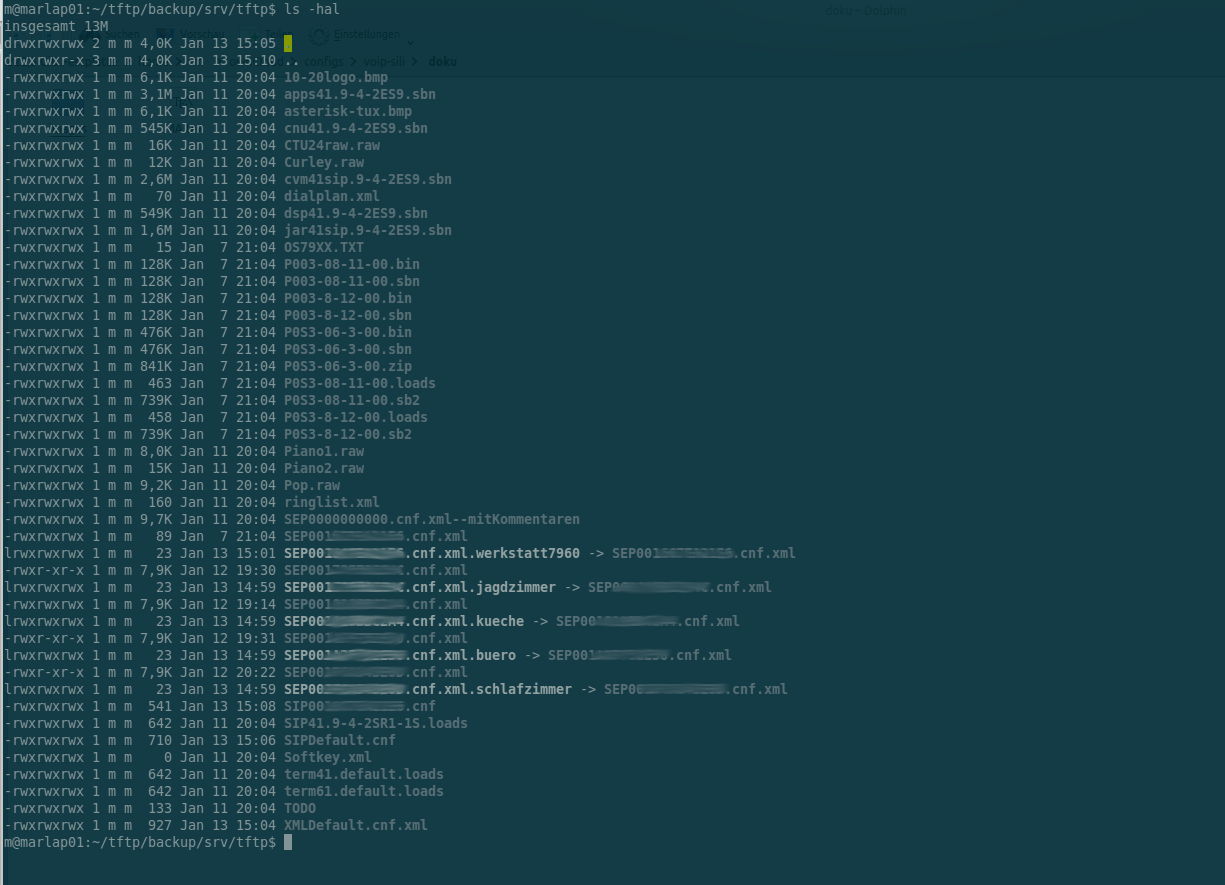
\includegraphics[width=1\hsize]{./images/atftpd-cisco7960-7961.png}
\end{center}
\caption[TFTP-Verzeichnis zu gleichzeitigen Nutzung von 7960 und 4x 7961 Telefonen.]
{\label{tftp79607961}TFTP-Verzeichnis zu gleichzeitigen Nutzung von 7960 und 4x 7961 Telefonen. Quelle:Autor}
\end{figure}


\subsection{Cisco 7962}
siehe Cisco 7961.

\end{document}




